\documentclass[a4paper,12pt]{article}

\usepackage{geometry}       % Required for page layout.
\usepackage{hyperref}       % Required for hyperlinks.
\usepackage{graphicx}       % Required for figures.
\usepackage{subfig}         % Required for minipages.


\usepackage{amsmath}
\usepackage{amsfonts}
\usepackage{amssymb}
\usepackage{amsthm}
\usepackage{float}

\usepackage{hyperref}
\usepackage{listings}
\usepackage{xcolor}

\definecolor{codegreen}{rgb}{0,0.6,0}
\definecolor{codegray}{rgb}{0.5,0.5,0.5}
\definecolor{codepurple}{rgb}{0.58,0,0.82}
\definecolor{backcolour}{rgb}{0.95,0.95,0.92}

\lstdefinestyle{mystyle}{
    backgroundcolor=\color{backcolour},   
    commentstyle=\color{codegreen},
    keywordstyle=\color{magenta},
    numberstyle=\tiny\color{codegray},
    stringstyle=\color{codepurple},
    basicstyle=\ttfamily\footnotesize,
    breakatwhitespace=false,         
    breaklines=true,                 
    captionpos=b,                    
    keepspaces=true,                 
    numbers=left,                    
    numbersep=5pt,                  
    showspaces=false,                
    showstringspaces=false,
    showtabs=false,                  
    tabsize=2
}

\lstset{style=mystyle}
\lstset{numbers =none}


\newgeometry{vmargin={25.4mm}, hmargin={27mm,27mm}}
\setlength\parindent{0pt}   % Disable paragraph indent.

\title{Cellular automaton traffic model of multilane highway}
\author{Axel Kierkegaard}
\usepackage{float}
\usepackage{makecell}
\begin{document}
\maketitle

\section{Introduction}
In a world heavily dependent on transportation between different areas, traffic modeling is an essential tool to enable development of correctly dimensioned infrastructure. To avoid traffic congestion on important roads an accurate description of reality is needed so that problems can be addressed beforehand. In this report the goal is to develop a model simulating a multilane highway, and comparing the traffic flow for a different number of lanes. Some of the questions we will investigate are:

\begin{itemize}
  \item \textbf{How does the road capacity compare for different number of lanes?}
  This is an important question when a traffic planner needs to use the knowledge of the traffic flow along a specific route to design a road with a sufficient number of lanes to carry that traffic.
  \item \textbf{For a multilane highway - how does the fraction of cars and flow rate in respective lanes depend on the density of cars?} There are some theories that the passing lanes, supposed to be the fastest moving, are actually slower in heavy traffic.\footnote{Los Angeles Times, https://www.latimes.com/archives/la-xpm-1992-04-13-me-189-story.html}
  \item \textbf{How does the distribution of velocities of the cars affect the flow rate, for different number of lanes?} The model will use cars with different maximum velocities. It is interesting to investigate how a more widely spread distribution of velocities affect the flowrate, and if the effect is the same for one lane as for several.
\end{itemize}

Furthermore, we will of course discuss statistical accuracy and discretization issues for the model, however that discussion will be introduced after the model itself has been described.

\section{Model description}
There are of course many different ways to implement a model of traffic flow, however here we will use a cellular automaton model using discrete time steps and a number of rules for the cars to follow. 

The system is initialized with a given road length and uses periodic boundary conditions so when a car reaches the end of the road it comes back to the beginning of it (meaning that the road system can be visualized as a circle). We will discuss later on the effect the road length has on the results. Furthermore, a simulation is here created with a fixed number of lanes and cars. This is a simplification since a normal highway has entries and exits for cars joining and leaving the highway, and in Sweden so called 2+1-roads are common where the number of lanes changes between 1 and 2 in each direction. The merges of lanes caused by these designs are often the cause of traffic congestion which is why a more accurate model definitely should take these effects into account.\\ 

Another important part of the model is the velocity distribution. To resemble real-life scenarios, we need the cars to have different maximum speeds. The velocities are approximately normally distributed according to some studies, \footnote{\url{https://www.sciencedirect.com/science/article/pii/S1877705817319318?ref=pdf_download&fr=RR-2&rr=787cc9874e7a991b}} and some swedish investigations have shown that almost 50\% drive too fast on certain roads.\footnote{\url{https://www.vibilagare.se/nyheter/40gata-da-kor-halften-for-fort}} Therefore, we will assume that the maximum speeds of the cars are normally distributed around the maximum velocity of the road. However, since the velocities as well as the positions need to be integers in this discrete model, we will have to round off to the closest integer for each velocity. It is a simplifcation to only allow discrete, integer values for the time, positions and velocities, but the model can still be meaningful.\\ 

Now let us go through the rules of the system, that determines the behavior of the cars. The rules, looped over all cars separately in this order are:

\begin{enumerate}
	\item If $v_i < v_{i, max}$ then increase the velocity of the car i, $v_i \rightarrow v_i+1$.\\
	Models the acceleration to the car's maximum velocity.
	\item Compute the distance from car i to the closest car in front, $d_f$. 
	\begin{enumerate}
		\item If car i is in the outermost lane and $v_i \geq d$, then the velocity needs to be reduced $v_i \rightarrow d-1$. 
		\item If car i is not in the outermost lane and $v_i \geq d$, calculate the distance to the closest car in front ($d_{fl}$) and behind it ($d_{bl}$) in the lane to the left. If $d_{fl}<d_f$ and $d_{bl}>v_{bl}$ car i will switch to the left lane. Here $v_{bl}$ is the velocity of the car behind in the left lane. 
This means that if there is more space in front in the left lane, and the space to the closest car in the back is bigger than the velocity of that car, car i will switch to that lane. No matter if it switches lanes or not, the velocity is then decreased if it is not smaller than the distance to the closest car in front, as in (a). 
		\item If car i is not in the innermost lane and $v_i < d$, calculate the distance to the closest car in front ($d_{fr}$) and behind it ($d_{br}$) in the lane to the right. If $d_{fr}>v_i$ and $d_{br} > v_{br}$ car i will switch one lane to the right. This essentially means that if there is enough space in the right lane and safe to switch lanes (no fast car in behind), the car will switch to that lane.
	\end{enumerate}
	
\item With probability p, decrease the velocity of car i, $v_i \rightarrow v_{i-1}$. This is only done when $v_i>0$. 
\item Update the positions so that $x_i(t+1) = x_i(t) +v_i$
\end{enumerate}

Let us further discuss these rules. Especially interesting are the rules for lane-changing, since this is quite a complex phenomenon and drivers are generally quite different in their behavior. It is reasonable that a driver switch lane to the left if there is more space there and the driver in front is driving too slow, and that they switch back to the right when there is enough space again. However, a more advanced model should also encompass that a driver can see more than just the distance to the car in front, the (approximated) velocities and cars further ahead are also taken into consideration when driving in real life. At the same time, a model fully implementing these factors as well would require more details of  decision making, sight conditions on the road etc. making the model far too complicated.\\

Another important condition for lane changing to be allowed is that the velocity of the closest car behind in the new lane is smaller than the distance to said car. This essentially means that no car will have to suddenly break because a car moves in front of it from another lane, which may be more of an ideal rather than an exact description of reality. In real life, there are of course some drivers who switch lanes forcing the car behind to break, but allowing cars to switch lanes without "checking behind" would cause nonphysical scenarios. For example, a car with a very low velocity (or even 0) could change lane causing a car behind to break from max speed to 0 in a single time step. To avoid these scenarios checking the car in the back is needed, even if it is not completely realistic that a driver can determine the exact velocity of the car behind.\\

In the third step, we reduce the velocity of a car with a given probability p. Too simulate a highway this probability should be rather low since cars generally try to uphold a constant velocity on highways. Again, the model could be improved by allowing this probability to change for different cars (or different lanes since cars in the passing lanes probably are less likely to break), but fir simplicity we have chosen to not do so in this model.\\

There are of course many more possible improvements for a traffic model, taking into account more complex factors in decision making - such as drivers trying to find an open spot in the right lane if a fast car approaches from behind, drivers slowing down to give another car the chance to enter the lane and so on. However, this model encapsulates the basic behaviors on a multilane highway and mentioned improvements will be left to future investigations. 

\section{Method}
The cellular automaton model uses discrete time steps, where the position and velocity of each car is updated according to the rules previously described. The parameters are the number of cars $n_{cars}$, road length L, probability for a car to reduce its velocity p and the velocity $v_{road}$. The maximum velocity of each car is taken as a sample from a gaussian distribution, with the mean $v_{road}$ and standard deviation 1 unless other specified. The results are rounded to closest integer, or to 1 if it is less than that.\\

The flow rate is defined as the sum of the cars velocities divided by the road length and is calculated for each time step. Furthermore, the proportion of cars in each lane is calculated as well as the mean velocity for cars in that lane.\\

We will also estimate the errors for our measurements of the observables. Assume we have independent observations $y_1, \dots, y_n$ (i.e. from different simulations), where y can represent for example the mean flow rate of the simulation. The mean $\bar{y}$ has a corresponding error of the mean $s_{\bar{y}} = \frac{s_y}{\sqrt{n}}$ where $s_y$ is the sample standard deviation 

\begin{equation}
	s=\sqrt{\frac{1}{n-1} \sum_{j=1}^{n}(y_j-\bar{y})^2}
\end{equation}

\subsection{Regression}
We will use the least-square-method to fit different models to our data. The coefficient of determination $R^2$ is given by

\begin{equation}
R^2 = 1 - \frac{SS_{res}}{SS_{tot}} = 1 - \frac{\sum_{i=1}^{n} (y_i-f(x_i))^2} {\sum_{i=1}^{n} (y_i-\bar{y})^2}
\end{equation} 

where $y_i$ is the measured data point at $x_i$ (total of n measurements), $f$ the fitted function.
 

\section{Results}
When simulating the system with 25 cars, road length 50, mean velocity $v_{road}=5$ for a 1,2 and 3 lane highway we achieve the plot in figure \ref{fig1} showing the flow rate as a function of time. There is an initial increase in the beginning (the acceleration phase) before the flow rate stabilizes. We can with good margin assume that the system is stable after 100 time steps. In table 1 the mean and difference between maximum and minimum of the flow rate is shown, calculated for the last 100 time steps. The flow rate oscillates very much, and more for the systems with several lanes than with a single one. Furthermore, the mean of the flow rate increases with an increased number of lanes, as to be expected. However, an interesting fact is that the flow rate is 3 times higher for 2 lanes and almost 5 times higher for 3 lanes compared to a 1-lane road. An explanation could be that the cars not only get more space with more lanes, but that it also enables a division of the faster and slower cars choosing different lanes.

\begin{figure}[H]
	\centering
        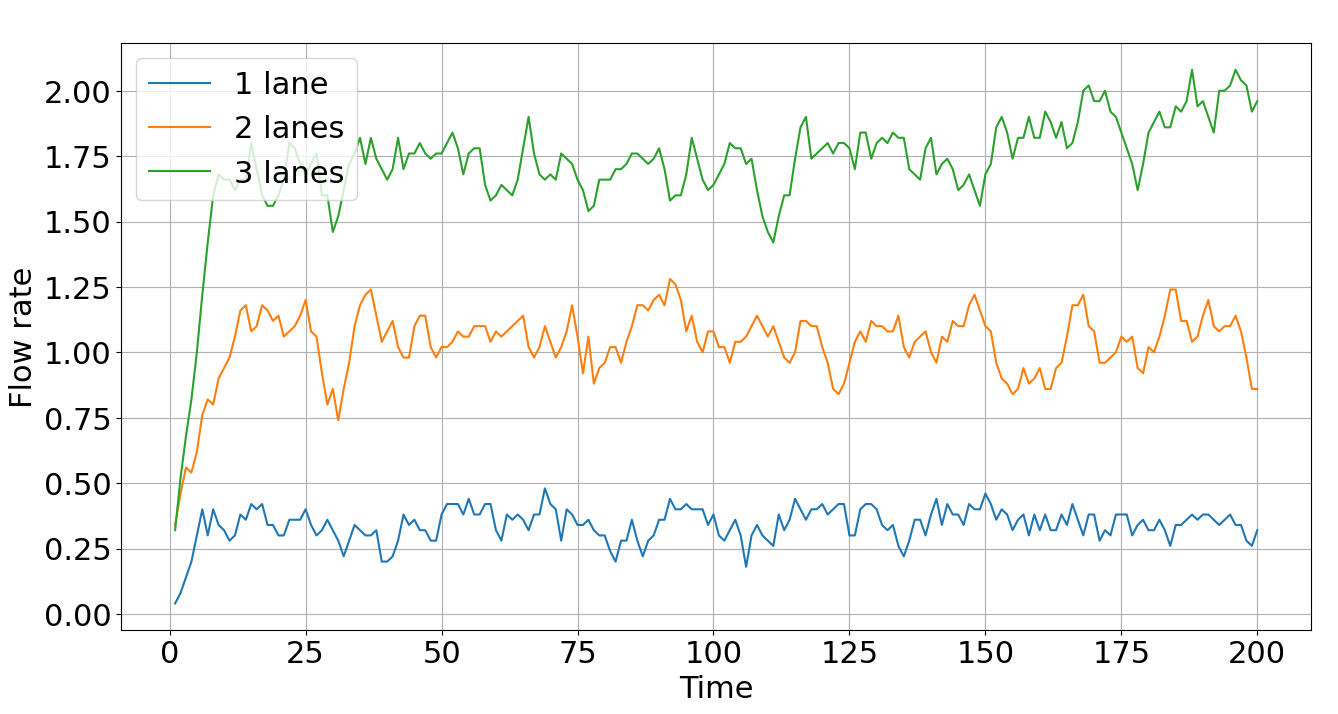
\includegraphics[scale=0.45]{fig1.png}
    \caption{Flow rate vs. time for different number of lanes, $n_{cars}=25$, L=50, $v_{road}=5$, p=0.2.}
    \label{fig1}
\end{figure}

\begin{center}
\def\arraystretch{1.5}
\begin{tabular}{ |c|c|c| } 
 \hline
	Number of lanes & \makecell{Mean of flow\\ (last 100 time steps)} & \makecell{Max flow - min flow\\ (last 100 time steps)}\\
 \hline
	 1 & 0.36 & 0.26 \\
	 2 & 1.08 & 0.46 \\
	 3 & 1.74 &  0.50 \\
 \hline
\end{tabular}\\
\end{center}
Table 1: Mean of flow and difference between maximum and minimum flow, calculated for the last 100 time steps for the simulation shown in figure \ref{fig1}.\\

In figure \ref{semq} we see the standard error of the mean flow rate as a function of the number of simulations. The error arises from the randomness in the assignment of max velocities and from the parameter p (breaking probability of a car). The error seems to be of the order of $10^{-2}$, and it decreases towards 0 with increased number of iterations as it should. We note that the error seems to be roughly the same for different number of lanes, and in the log-log-scaled plot we see that all of the errors approximately decreases $\propto \frac{1}{\sqrt{n}}$.

\begin{figure}[H]
	 \centering
    \begin{minipage}{.5\textwidth}
        \centering
        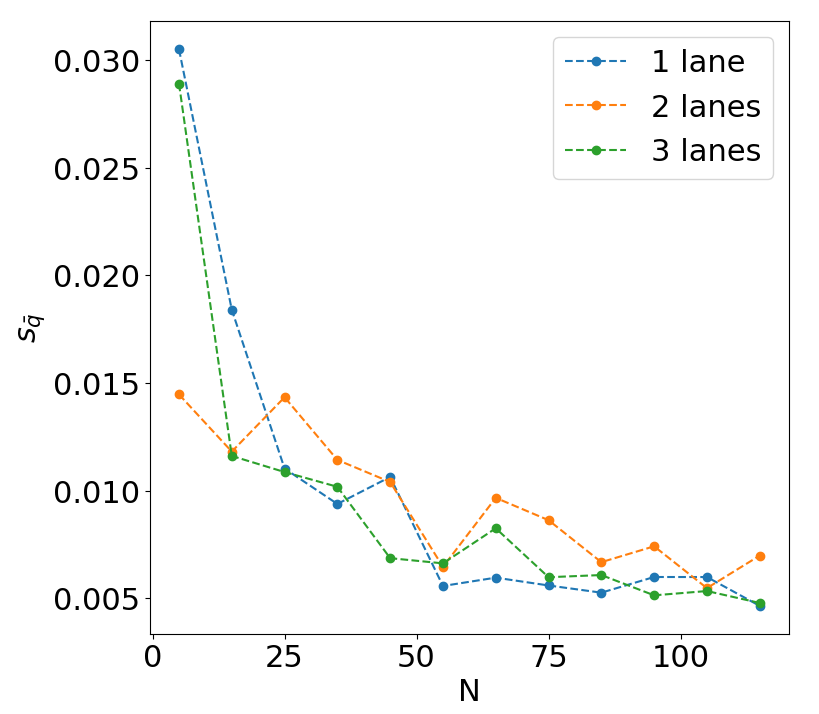
\includegraphics[width=8cm]{fig6.png}
        \captionof*{figure}{Normal scale}
    \end{minipage}%
    \begin{minipage}{.5\textwidth}
        \centering
        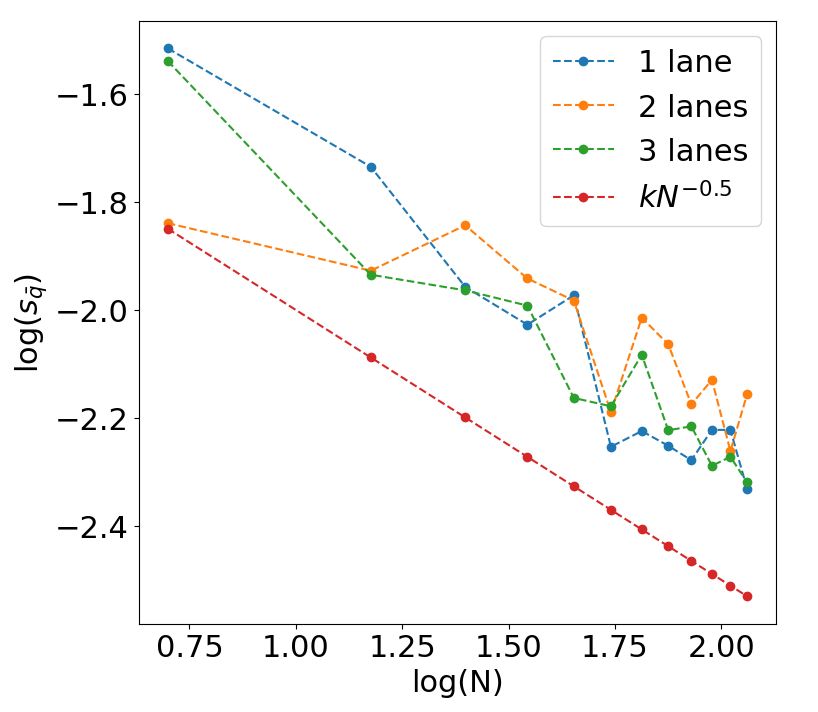
\includegraphics[width=8cm]{fig7.png}
        \captionof*{figure}{Logarithmic scale}
    \end{minipage}
    \caption{Standard error of the mean flow rate $s_{\bar{q}}$ as a function of number of simulations N. L=100, $n_{cars}=20$, p=0.2, $v_{road}=5$. A line $kN^{-0.5}$, (k is a suitable constant), is fitted to show the rate of decline.}
    \label{semq}
\end{figure}

\subsection{Fundamental Diagram}
The fundamental diagram of flow rate plotted against density of cars is an essential tool in traffic flow analysis. Here we will try to fit a suitable model to describe the flow rate as a function of density. One of the oldest used models is the Greenshields model, which states that the flow rate depends on density as a second degree polynomial.\footnote{\url{https://research.chalmers.se/publication/527726/file/527726_Fulltext.pdf}} In figure \ref{fig3} we have generated the fundamental diagram by simulating the system for different number of cars (where density $\rho = \frac{n_{cars}}{L}$) and calculating the flow rate. For each point the flow rate is calculated as the mean of 10 simulations, and the flow rate from a simulation is taken as the mean over the last 100 time steps. The fitted second degree polynomials are shown in table 2, and we see that it is not a good fit at all, which the low $R^2$-values also are indicators of. Greenshields model fails to describe the behavior of the fundamental diagram in this simulation and we will therefore discard it without further discussion.\\

\begin{figure}[H]
	\centering
        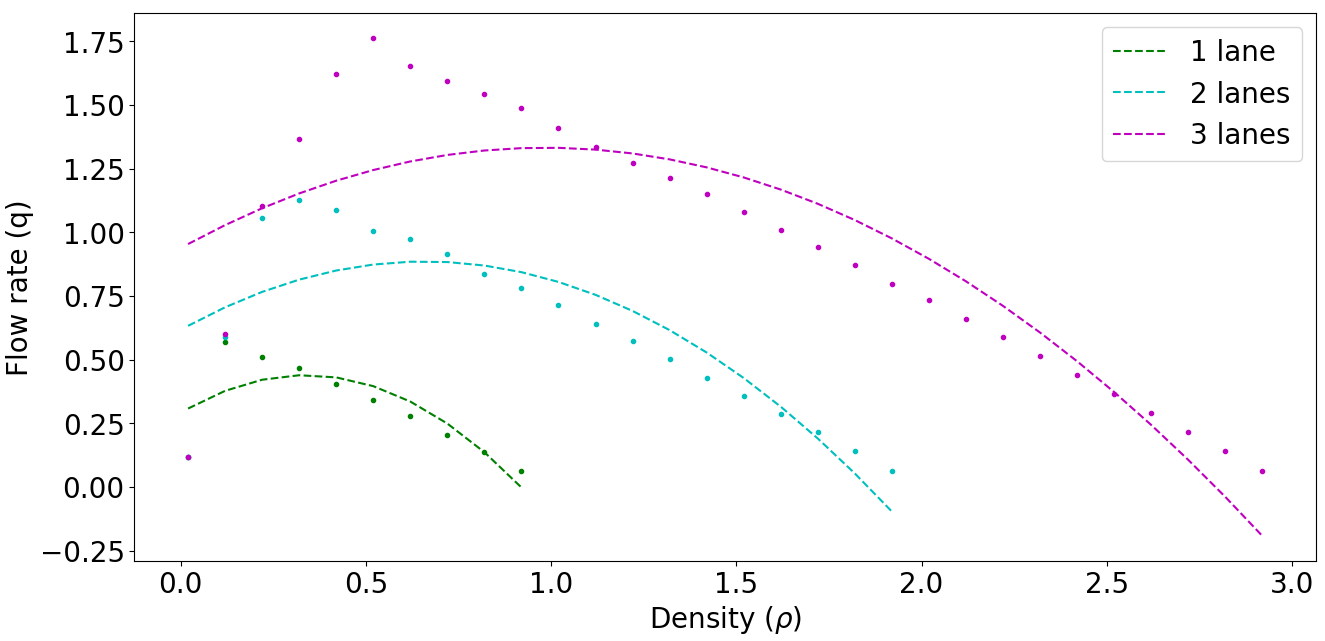
\includegraphics[scale=0.45]{fig3.png}
    \caption{Flow rate vs. density for different number of lanes, L=50, $v_{road}=5$, p=0.2.}
    \label{fig3}
\end{figure}

\begin{center}
\def\arraystretch{1.5}
\begin{tabular}{ |c|c|c| } 
 \hline
	\makecell{Number of\\ lanes} & Regression curve & $R^2$ \\
 \hline
	 1 & $q= -1.30\rho^2+0.88\rho+0.29$  & 0.66016  \\
	 2 & $q= -0.62\rho^2+0.82\rho+0.62$ & 0.71849 \\
	 3 &$ q= -0.51\rho^2+0.81\rho+0.94 $& 0.73947 \\
 \hline
\end{tabular}\\
\end{center}

Another commonly used model is the triangular diagram, which models the fundamental diagram with two linear functions. In figure \ref{fig2} we have, for different number of lanes, fitted one line for the points before the maximum recorded flow rate, and one line for the remaining part. The equations are shown in table 3, together with the $R^2$-values (calculated for the entire triangular curve, all points) which are very close to 1. This confirms what also can be seen in the figure, that the fit is very good.\\

The flow rate approaches 0 for $\rho=1$ with one lane, $\rho=2$ with two lanes and so on, which is to be expected as that means the roads are completely full. It is also expected that q=0 when $\rho=0$. Furthermore, we see that the maximum flow rate more than doubles when going from 1 lane to 2, and it more than triples when going from 1 to 3. The critical density (where the flow rate starts to go down) also increases with more lanes as can be seen in table 3. Another interesting fact is that the regression lines seem to be almost parallel for different number of lanes, with the big difference being the constant added to the line describing the decrease of flow rate. 
\begin{figure}[H]
	\centering
        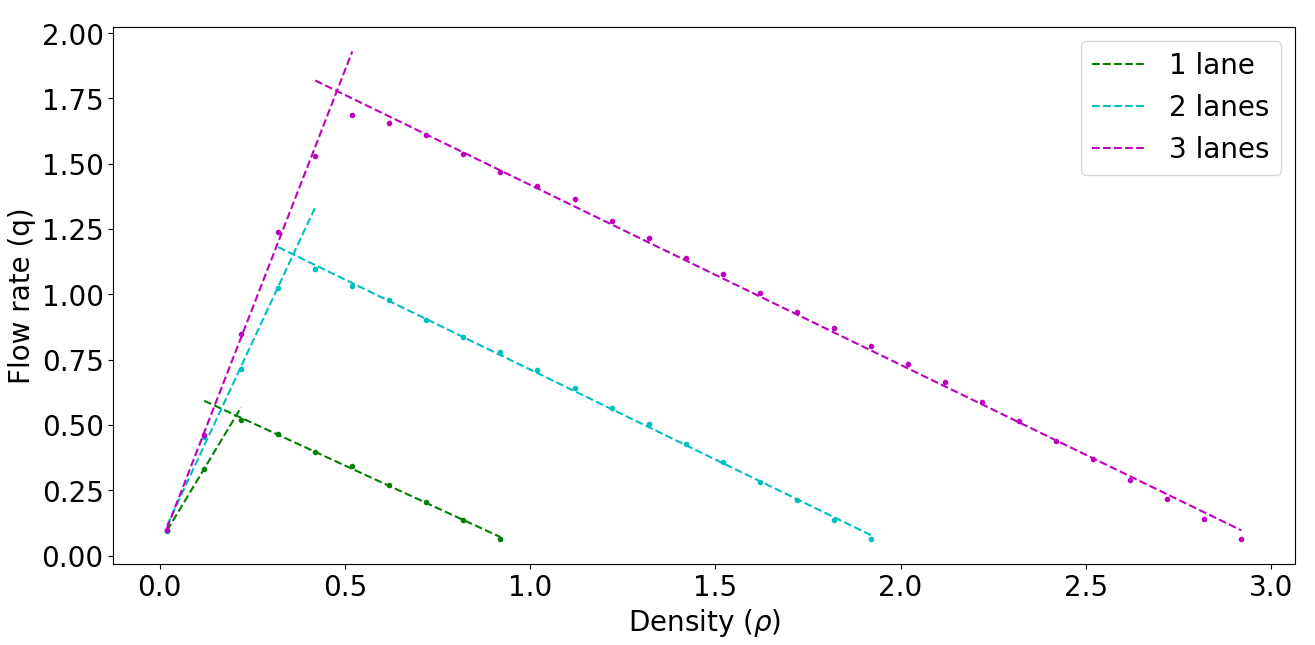
\includegraphics[scale=0.45]{fig2.png}
    \caption{Flow rate vs. density for different number of lanes, L=50, $v_{road}=5$, p=0.2. For each point the flow rate is calculated as the mean of 10 simulations, and the flow rate from a simulation is calculated as the mean over the last 100 time steps.}
    \label{fig2}
\end{figure}

\begin{center}
\def\arraystretch{1.5}
\begin{tabular}{ |c|c|c|c|c|c| } 
 \hline
	\makecell{Number of \\lanes} & \makecell{Critical\\ density} &\makecell{Max flow rate \\ (predicted)} & \makecell{Regression curve \\(increase)} & \makecell{Regression curve \\(decrease)} & $R^2$ \\
 \hline
	 1 & 0.207 & 0.536 &$q=2.36\rho+0.049$ & $q=-0.65\rho+0.67$ & 0.99857  \\
	 2 & 0.361 & 1.15 &$q=3.04\rho+0.055$ & $q=-0.69\rho+1.40$  & 0.99851 \\
	 3 & 0.478 & 1.78 &$q=3.65\rho+0.033$ & $q=-0.69\rho+2.11$ & 0.99823 \\
 \hline
\end{tabular}\\
\end{center}


\subsection{Proportion and velocity of cars in different lanes}

Simulating a 2-lane road for different densities, we can see (figure \ref{fig45}) that for low densities the majority of the cars are in the inner lane (seems reasonable - no need for overtaking on an empty road). However, the share of cars in the second lane increases rapidly and for densities 0.5 and above there are roughly the same number of cars in both lanes, and the second lane even shows a tendency to be a bit more crowded. Furthermore, for low densities the mean velocity is higher, however for densities above 0.5 the mean velocity is the same or lower in the second lane compared to the first. This indicates that the passing lane is not faster in a traffic jam. 
\begin{figure}[H]
	 \centering
    \begin{minipage}{.5\textwidth}
        \centering
        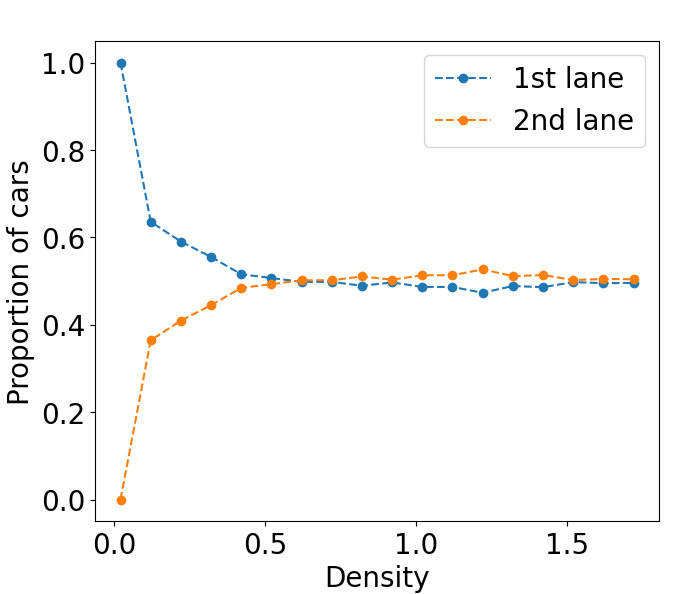
\includegraphics[scale=0.37]{fig5.png}
        \captionof*{figure}{Proportion of cars in lane vs. density}
    \end{minipage}%
    \begin{minipage}{.5\textwidth}
        \centering
        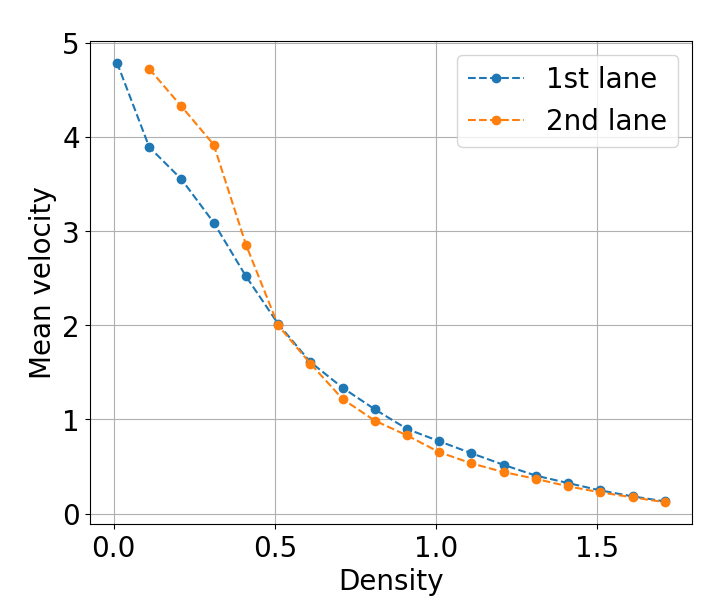
\includegraphics[scale=0.37]{fig4.png}
        \captionof*{figure}{Mean velocity in respective lane.}
    \end{minipage}
    \caption{Proportion and mean velocity of cars in 1st (inner) and 2nd (outer) lane for a 2-lane highway with L=50,$v_{road}=5$, p=0.2. Mean of 10 simulations for each density is used.}
    \label{fig45}
\end{figure}

For 3 lanes the behavior is similar. With few cars only the first lane is filled and as the road becomes more crowded the second and third lane become more populated (the third more slowly though). For high densities there seems to be a uniform distribution of cars among the three lanes, and while the mean velocity is higher in the second and third lane for low densities, they seem to be the same when the road is crowded.
\begin{figure}[H]
	 \centering
    \begin{minipage}{.5\textwidth}
        \centering
        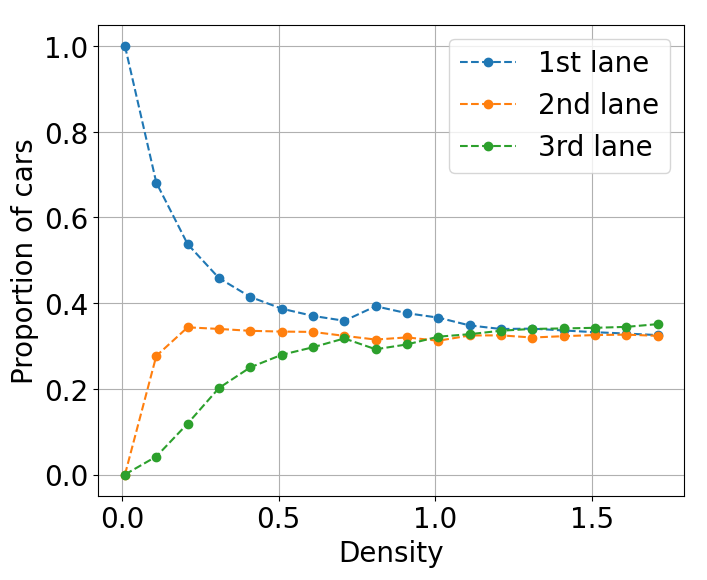
\includegraphics[scale=0.37]{fig8.png}
        \captionof*{figure}{Proportion of cars in lane vs. density}
    \end{minipage}%
    \begin{minipage}{.5\textwidth}
        \centering
        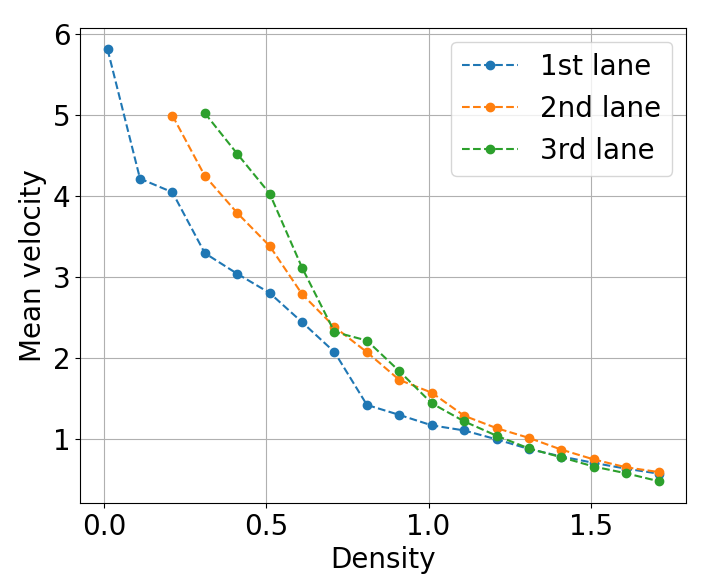
\includegraphics[scale=0.37]{fig9.png}
        \captionof*{figure}{Mean velocity in respective lane.}
    \end{minipage}
    \caption{Proportion and mean velocity of cars in 1st (inner), 2nd (middle) and 3rd (outer) lane for a 2-lane highway with L=50,$v_{road}=5$, p=0.2. Mean of 10 simulations for each density is used.}
    \label{41a}
\end{figure}

We have previously analyzed the error for the flow rate, now let us do the same for the proportion and mean velocity. In figure \ref{sempv} below we see the SEM for the proportion of cars in the inner lane and the mean velocity in respective lane for a 2-lane road (using a log-log-scale). Similarly as before the errors decrease as $N^{-0.5}$. For the proportion the SEM is in the order of $10^{-2.3} = 0.005$ while for the mean velocity the SEM is around $10^{-1.4} = 0.04$ for 10 simulations as was used for each point in the diagrams above. 
\begin{figure}[H]
	 \centering
    \begin{minipage}{.5\textwidth}
        \centering
        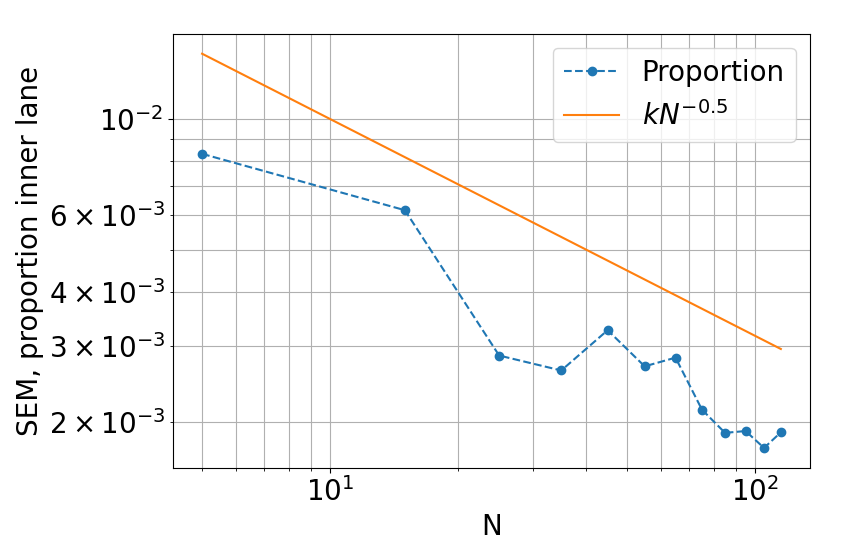
\includegraphics[scale=0.38]{fig11.png}
        \captionof*{figure}{Normal scale}
    \end{minipage}%
    \begin{minipage}{.5\textwidth}
        \centering
        \includegraphics[scale=0.38]{fig12.png}
        \captionof*{figure}{Logarithmic scale}
    \end{minipage}
    \caption{SEM for proportion of cars in inner lane and mean velocity in respective lane for a 2-lane road, as a function of number of simulations N. L=50, $n_{cars}=25$, }
    \label{sempv}
\end{figure}


\subsection{Effect of velocity distribution on flow rate}

\begin{figure}[H]
	\centering
        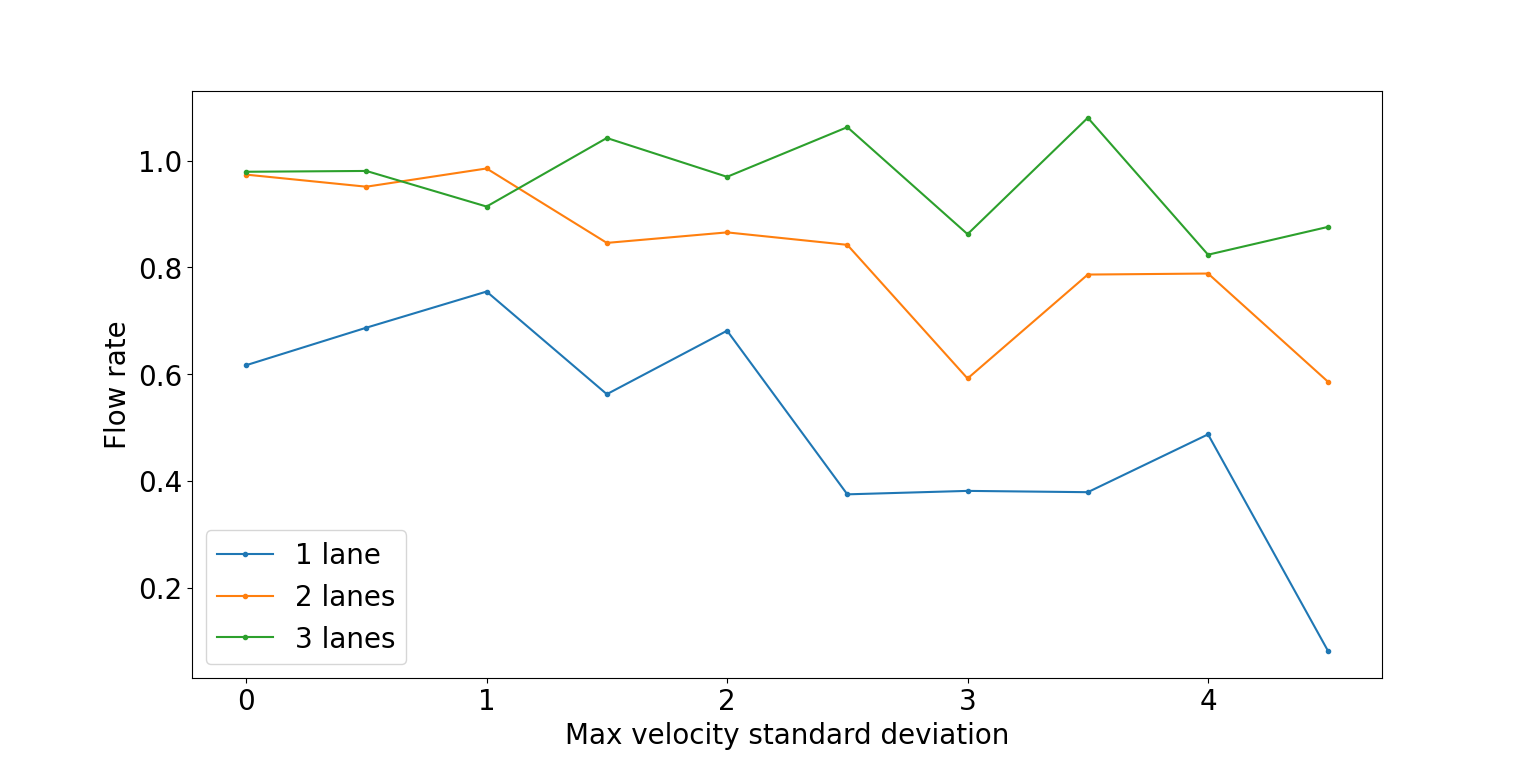
\includegraphics[scale=0.45]{fig10.png}
    \caption{Flow rate as a function of the maximum velocity standard deviation for a system with L=100, $n_{cars}=10$, p=0.2 and different number of lanes.}
    \label{fig10}
\end{figure}


\section*{Discussion}
Accuracy, precision, should have done more iterations. Avoiding changing velocities would increase precision but less accurate. 


\section{Appendix - Python code}

\lstinputlisting[language=python]{codelistings.py}

 

\end{document}